\chapter{Developer Documentation}
\label{ch:developer}

The main aim of this application is to be expanded by developer to accommodate the needs of the farmer as 
well as the method and procedures developed by the data analysts.
The application is composed of many interconnected components which work together to process data end-to-end.
The developer is assumed to have some knowledge about web frameworks and databases.

\section{Prerequisites}
The developer should have the following installed in their environment:
\begin{itemize}
    \item AgrifoodIT project repository \cite{github_repo}
    \item Git version control system \cite{git}
    \item Redis NoSQL database \cite{redis}
    \item PostgreSQL database \cite{postgresql}
    \item Celery \cite{celery}
    \item Python
    \item Python packages in requirements.txt file
    \item PyCharm IDE or any other IDE as per preference
\end{itemize}

\begin{note}
	The file \texttt{AgrifoodIT/settings.py} should be updated with the credentials and port of PostgreSQL, Celery and Redis.
\end{note}

The database needs to be populated and the following commands should be run in the 
project folder in the order listed:
\begin{itemize}
    \item python manage.py createsuperuser
    \item python manage.py migrate
\end{itemize}

To run the project on localhost use the command \texttt{python manage.py runserver}.

\section{Libraries}
\label{sec:libaries}

\subsection{Django}
Django is the most popular and powerful python web application frameworks. It comes already with many
features built in so that the project can be set up and running without much external support. 
It uses the MVT (Model View Template) architecture and some of the built in features are listed below:

\begin{itemize}
    \item Object Relational Mapper: Maps objects written in code to the database.
    \item URL Routing: Automatically calls correct method based on the URL request.
    \item Django Admin: GUI interface for interacting with the database.
    \item Templating Engine: Combines the data from controller with the view.
    \item Safe and Secure Authentication Module
\end{itemize}

\begin{definition}
	Model is codified interface of data. The logical data structure is defined here and it is represented in the database
	automatically by the ORM.
\end{definition}

\begin{definition}
	Template is the front-end or the user interface. Templates are saved in HTML/CSS/JavaScript files. The templating engine combines
	templates with the data from the view. Templates can be broken into several components and combined as per the request by the template engine.
	For example the navigation bar is a separate template which is included in each page.
\end{definition}

\begin{definition}
	View is the logical part of the program. It ingests data and manipulates data for output. It glues the Model and the Template.
\end{definition}

A Django project is composed of multiple apps each having their own set of MVT. Each app is pluggable as it can be removed from the project
without crippling the project itself. An app can be defined as a large component with a specific goal which can exist on it's own.
In this project apps from other projects and from the web can be imported for faster development. A top-level MVC can be defined as well which can be
shared by the apps. Our project is composed of 2 apps:
\begin{itemize}
    \item Dashboard: Data Input, Processing and Storage.
    \item Analysis: Visualization
\end{itemize}

Further explanation about the apps is given in the sections \ref{sec:models},
\ref{sec:views} and \ref{sec:templates}. Each app in the project initially
starts with the same project structure. The migration folder contains files
which hold the changes to be made to the database to implement the models
defined in \texttt{models.py}. For the template files they have to be saved in a
folder with the same name as the app itself inside a "templates" folder in the
app directory. This is so that when Django scans the whole project for templates
it separates the templates according to the folder in which they were found and
not under which app folder they were found. If this is not used then Django will
fail to see the template files and one cannot reference them in their code. For
celery tasks they are saved in \texttt{tasks.py} folder. The \texttt{urls.py}
file holds the routing information for the app. Here the URLs are attached to
the respective views from \texttt{views.py} file. Further more if a URL has to
accept parameters it is also done in this file. For example when re-processing
an uploaded file we send the primary ID of the file as a URL parameter and it is
defined as follows \texttt{weather\/process\/<int:id>}. Each defined URL is
given a name which is referenced in template files. This allows flexibility when
URL changes have to take place then it can be done in the URL file only without
modifying the template files as they will be dynamically updated by Django.

The static folder contains minified CSS and JavaScript files. In a template if
it is necessary to load all static files before further processing the static
tag can be used. \texttt{Manage.py} file is Django's script for
starting/modifying/creating the project and it's apps. It can also be used to
create a python shell for quick prototyping. The requirements text file contains
all the Python packages required by the project to work. It should be updated
incase a new package has been installed. It is preferable to manually update the
requirements file as usually the dependencies are not included and only the core
packages are listed.

\begin{figure}[H]
	\dirtree{%
	.1 /.
	.2 AgrifoodIT. 
		.3 celery.py. 
		.3 settings.py. 
		.3 urls.py. 
	.2 analysis. 
		.3 migrations.
		.3 templates/analysis. 
		.3 models.py. 
		.3 tasks.py. 
		.3 urls.py. 
		.3 views.py. 
	.2 dashboard. 
		.3 migrations.
		.3 templates/dashboard.
		.3 models.py. 
		.3 tasks.py. 
		.3 urls.py. 
		.3 views.py. 
	.2 static. 
	.2 templates. 
	.2 manage.py. 
	.2 requirements.txt. 
	}
	\caption{Directory structure of the project}
	\label{fig:directory_structure}
\end{figure}

One of the most powerful parts of Django is the automatic admin interface. It
reads metadata from your models to provide a quick, model-centric interface
where trusted users can manage content on of the database. It’s not intended for
building your entire front end around. \cite{django_admin}. The admin interface
can be accessed by \texttt{localhost:port\textbackslash admin} URL. All models which have
been registered in admin.py files in each app will automatically show up in the
admin panel. From there it is possible to manipulate all attributes of each
instance of the models saved in the database. The admin interface is password protected and
the credentials created during the command \texttt{createsuperuser} are to be used for access.
Within the admin interface one can configure additional users for access.

\begin{figure}[H]
	\centering
	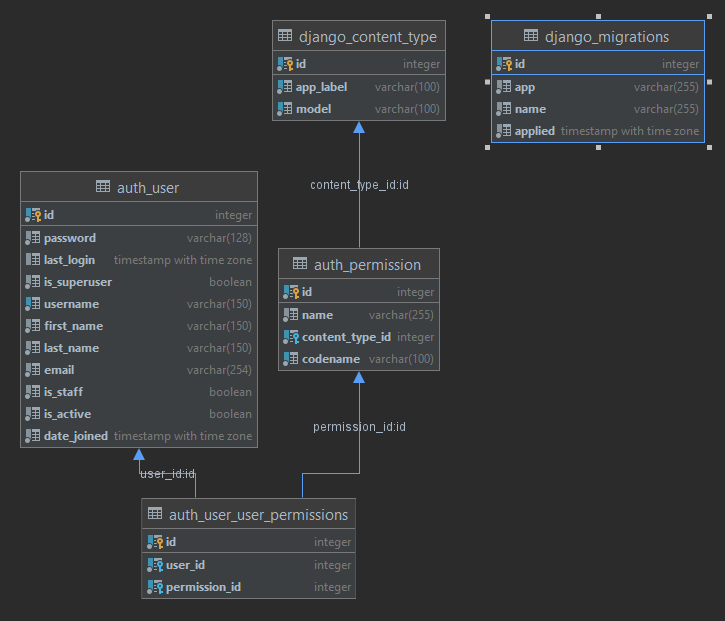
\includegraphics[width=1.0\textwidth]{erd_django}
	\caption{ERD diagram for Django database tables}
	\label{fig:erd_django}
\end{figure}

\subsection{Celery}
Celery is the background task processor used in the project. The purpose is to
have data and process intensive tasks to be delegated to runners in the
background. These tasks continue to run until their completion without affecting
the performance of the web application. On a system one can run as many
instances of runner as required. If a runner is not available the tasks are
saved in the database and later sent when runners are available. The first
parameter is the name of the project defined in the celery instance instantiated
in celery.py file. The log level is set to information level. To run a celery
runner on windows it is necessary to set the pool flag to solo otherwise it will
not run as celery is not officially supported on windows platform. On other
platforms this flag is not necessary.

\lstset{caption={Command to run an instance of a celery runner in cmd/bash}}
\begin{lstlisting}[language={bash}]
	celery -A AgrifoodIT worker -l info --pool=solo
\end{lstlisting}

Celery automatically distributes the tasks between the available runners. Each
runner communicates with the project celery instance through Redis. Celery
settings file (AgrifoodIT\textbackslash celery.py) contains the method
\texttt{app.autodiscover\_tasks()} which scans the whole project for decorated
methods and automatically registers them as celery tasks.

Celery tasks are python methods with the decorator \texttt{\@shared\_task()}. The normal rules of python methods apply here. It is not always
necessary to return a status message but it is helpful in debugging. In the project
tasks for the dashboard app are defined in the file \texttt{dashboard/tasks.py}.

The celery task finds the uploaded file using the primary key and then calls the
method for further processing of the file. The file contents are extracted and
each line is processed. If successful the lines are converted into Django models
and uploaded to the database.

\lstset{caption={Celery task to process weather files}, label=src:processNewWeatherFile}
\begin{lstlisting}[language={Python}]
@shared_task()
def processNewWeatherFile(primary_key):
	file = WeatherFile.objects.get(pk=primary_key)
	print(f'===== {file.file_name} ===== START')
	process_weather_file(file.id)
	print(f'===== {file.file_name} ===== DONE')
	return {"status": True}
\end{lstlisting}

When a file is uploaded the respective view is triggered. This view creates a
new entry in the database saving the uploaded file. Then the view enqueues the 
celery task so that the file is processed in the background.

\lstset{caption={Enqueue a task asynchronously using delay method (Line 4)}, label=src:weather_upload}
\begin{lstlisting}[language={Python}]
def weather_upload(request):
if request.method == 'POST':
	text_file = request.FILES.get('file')
	file = WeatherFile.objects.create(file_name=text_file.name, processing_status=False, upload=text_file)
	processNewWeatherFile.delay(file.id)
	return JsonResponse({'status': 'success'})
return JsonResponse({'status': 'error'})
\end{lstlisting}

Celery automatically stores the enqueued tasks in the database and as soon as a runner is available they are run.
In the runner console we can see the status and output of each task.\ref{fig:celery-task-log}

\begin{figure}[H]
	\centering
	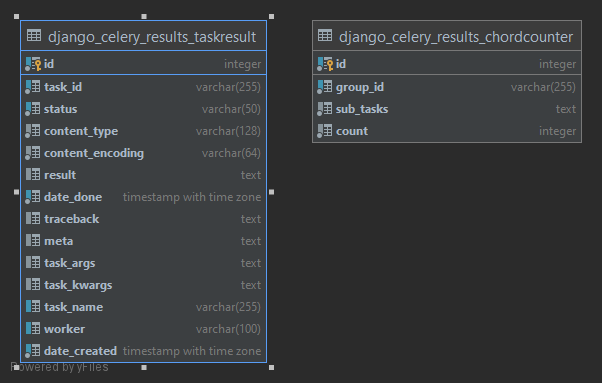
\includegraphics[width=1.0\textwidth]{erd_celery}
	\caption{ERD diagram for Celery task database tables}
	\label{fig:erd_celery}
\end{figure}

\subsection{Django-plotly-dash}
This is a package composed of 2 components Plotly and Dash. Plotly is graphing
library and Dash is responsive visualization platform. Using a graphing library
alone would require to write pythonic code to make the visualizations
interactive. Using Dash we can add interactivity to Plotly graphs using pre-built components such as
DateTime picker and using callbacks to update the graph based on the value of input components. Furthermore
Dash has online tools available which help to visualize data easily and then
generate python code automatically which can be used in our project with little
modification.\cite{plotly_chart_studio} 

In the project bar charts and 2 Y-Axis
scatter plot are implemented. \ref{fig:rohit-analysis}
The simple Temperature/Humidity graph is implemented as a Dash app. First we initialize the Dash app
by calling the constructor along with the name of the Dash app. This name can now be used through out the whole
project to refer to the Dash app. It is necessary to keep this name unique. We also provide a CSS document
which will modify the appearance of the HTML components. It is possible to find CSS documents online which 
can be used directly in the Dash app. Each graph is contained in a Figure class. To activate the second y-axis on a scatter plot
we have to set the secondary\_y parameter to true. Next the labels are set up for the graph and it's axes.
To set up a auto ranging label which will automatically populate with values based on the input data we can use the tickformat parameter.
This is used for the x-axis as based on the time data we can populate the x-axis without hardcoding the values. 

\lstset{caption={Dash app graph initialization},label=src:simpleexample_visualization}
\begin{lstlisting}[language={Python}]
app = DjangoDash('SimpleExample', external_stylesheets=external_stylesheets)
fig = make_subplots(specs=[[{"secondary_y": True}]])
fig.update_layout(title_text="Hourly Temperature vs Humidity")
fig.update_yaxes(title_text="Temperature Axis", secondary_y=False)
fig.update_yaxes(title_text="Humidity Axis", secondary_y=True)
fig.update_xaxes(title_text="Hour",tickformat="%I %p")
\end{lstlisting}

By adding a DateTime picker to the app layout and adding a callback to it we can
update the graph and show the data pertaining to a certain day. This thus makes
it a interactive graph which the user can update itself. We can add filter
parameters to the DateTime picker to limit the time period from which the date
can be picked. This can be further improved by querying the database for the
oldest and latest available data and using that as a time period. The html.Div
method will generate the HTML code necessary to show the elements on the web
page. Both elements are given their id's so that they can referred to in the
callback. To make sure that the DateTime picker shows up as a modal form we have
to set the with\_portal parameter to true otherwise the DateTime picker will
fill the full screen with itself. Here we can also set the initial value of any
component. However since there is a callback set up for these components, as the
app initializes the callback function will be triggered and the initial value
will be overridden by the return value of the function. In this case it is
preferable to set initial values for input components and dummy values for
output components. The figure variable for the scatter plot contains dummy data
and as the app the callback function creates a new graph figure from data from
the database. 

\lstset{caption={Adding components to Dash app layout}, label=src:dash_layout}
\begin{lstlisting}[language={Python}]
app.layout = html.Div([
	dcc.DatePickerSingle(
		id='my-date-picker-single',
		min_date_allowed=datetime.date(1995, 8, 5),
		max_date_allowed=datetime.date(2022, 9, 19),
		with_portal=True,
		date=datetime.date(2020, 8, 25)
	),
	dcc.Graph(id="scatter-plot", figure=fig)
])
\end{lstlisting}

In Dash, the inputs and outputs of our application are simply the properties of
a particular component. Whenever an input property changes, the function that
the callback decorator wraps will get called automatically. Dash provides the
function with the new value of the input property as an input argument and Dash
updates the property of the output component with whatever was returned by the
function. When the Dash app starts, it automatically calls all of the callbacks
with the initial values of the input components in order to populate the initial
state of the output components. Frequently we'll update the children of a
component to display new text or the figure of a dcc.Graph component to display
new data, but we could also update the style of a component or even the
available options of a dcc.Dropdown component. \cite{dash_basic_callbacks}

The callback uses the input of the DateTime picker to output to the graph. We
set the input and output variable names for the components. We retrieve values
from the database table according to the values selected in the DateTime picker
and then we represent the data in a Pandas data frame. The data from Weather
model has to be converted from a QuerySet to a list as Pandas does not accept
QuerySet type. The graph figure is set to update the graph within 500
milliseconds. This results in a smooth visual transition to the new plot. This
figure variable is returned to the scatter graph which figures out automatically
how to plot the data.

\lstset{caption={Interactivity using a DateTime picker}, label=src:dash_callback}
\begin{lstlisting}[language={Python}]
@app.callback(
	dash.dependencies.Output('scatter-plot', 'figure'),
	dash.dependencies.Input('my-date-picker-single', 'date'))
def update_figure(date_value):
	if date_value is not None:
		date_object = datetime.date.fromisoformat(date_value)
		df = pd.DataFrame(list(Weather.objects.filter(timestamp__date=date_object).values('timestamp', 'temperature','humidity')))
		fig.data = []
		fig.add_trace(go.Scatter(x=df['timestamp'], y=df['temperature'], name="Temperature"),secondary_y=False,)
		fig.add_trace(go.Scatter(x=df['timestamp'], y=df['humidity'], name="Humidity"),	secondary_y=True,)
		fig.update_layout(transition_duration=500)
		return fig
\end{lstlisting}

\begin{note}
	Each Dash app has to be declared in the \texttt{urls.py} file for it to be initialized. Without this initialization it cannot be
	used in the template.
\end{note}

The main benefit of using a Dash app is that we can use the components provided by Dash and we do not need to have to write
our own HTML/JavaScript code as it is all generated by Dash itself. The template thus becomes very simple as seen in code 
block \ref{src:simpleexample_template}. We just need to reference the Dash app by it's ID. The size can be controlled by the ratio
parameter. All Dash apps included in this manner are IFrames in the web page.

\lstset{caption={Include the Dash app in a template}, label=src:simpleexample_template}
\begin{lstlisting}[language={Python}]

<div class="" style="height: 100%; width: 100%">
	
</div>
\end{lstlisting}

One of the downsides of a Dash app is that there can only be a single instance of it. If multiple instances are needed such
as showing graphs of data relating to each pig we have to use Plotly apps.
Furthermore if one needs to leverage more power as provided by Django Views then it is recommended to use a Plotly app.
An example of a Plotly app is shown in section \ref{sec:fpmining_example}.

\begin{figure}[H]
	\centering
	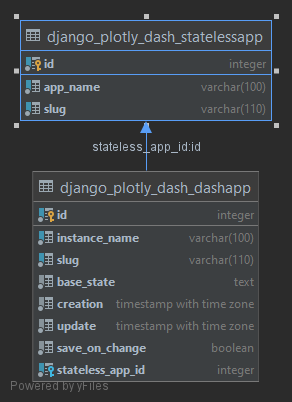
\includegraphics[width=0.5\textwidth]{erd_dash}
	\caption{ERD diagram for Django\_Plotly\_Dash database tables}
	\label{fig:erd_dash}
\end{figure}

\section{Models}
\label{sec:models}
In Django a model is a Python class which represents the definition of your data. 
The attributes of this class are a single database field. Each python class maps to a single database table.
In our project we implement 4 models so that we can process the 2 currently available types of input of movement and weather.

\begin{note}
	In each model listed the primary key is an auto incrementing integer. If this default key is used then it does not need to be
	explicitly defined in the model. The primary key for file models is also an incrementing integer because currently PostgreSQL does
	not support a FileField as a primary key.
\end{note}

\subsection{Pig model}
Each pig has a rfid tag in each ear thus we need to store 2 RFID strings. A nickname attribute is used as RFID is too difficult to
use in the application as an identifier for the user. Here the model can be extended with more attributes about the pig. This model
is pre-populated by Django in the database by a seed migration.

\lstset{caption={Pig model},label=src:pig_model}
\begin{lstlisting}[language={Python}]
class Pig(models.Model):
	rfid_A = models.CharField(max_length=200, unique=True)
	rfid_B = models.CharField(max_length=200, unique=True)
	weight = models.IntegerField(default=-1)
	nickname = models.CharField(max_length=50)
\end{lstlisting}

\subsection{Presence and Weather file models}
It is necessary to store each uploaded file in the database as when it comes to processing it will be a very resource intensive task
which can be offloaded to Celery runners in the background. Furthermore it is much easier to interact with files in the database compared to
manipulating files stored directly on disk and using I/O library of Python.

Both models are very similar in attributes. There is a need to show if the file
has been processed by a runner so the attribute \texttt{processing\_status} is
used. Other attributes are the metadata of the file and the upload field takes
the path where the file will be stored on disk. The file\_name field is set to be
unique as if the user uploads an existing file an error will occur which will
result in a unsuccessful upload. The error will be shown by the upload form.

\lstset{caption={File Upload models},label=src:file_models}
\begin{lstlisting}[language={Python}]
class PresenceFile(models.Model):
    file_name = models.CharField(max_length=200, unique=True)
    comments = models.CharField(max_length=200)
    processing_status = models.BooleanField()
    upload = models.FileField(upload_to='uploads/presence/')
class WeatherFile(models.Model):
    file_name = models.CharField(max_length=200, unique=True)
    comments = models.CharField(max_length=200)
    upload_date = models.DateTimeField('date uploaded', auto_now_add=True)
    processing_status = models.BooleanField()
    upload = models.FileField(upload_to='uploads/weather/')
\end{lstlisting}
	
\subsection{Presence model}
A sample of the data in a presence file is shown in code block \ref{src:presence_line}. Each line consists of:
\begin{itemize}
    \item Entry (+) or Exit (-) from the area
    \item Area/Reader number
    \item RFID of the pig
    \item Timestamp
\end{itemize}

\lstset{caption={},label=src:presence_line}
\begin{lstlisting}[language={}]
+ 1 E2000019991100851580391E 2020-07-13T17:17:35.321 
- 1 E2000019991100851580391E 2020-07-13T17:17:40.325 
+ 1 E2000019991100851580391E 2020-07-13T17:18:47.076 
- 1 E2000019991100851580391E 2020-07-13T17:18:52.078 
\end{lstlisting}

The data model for the above input is below. There are 2 foreign keys. The pig\_rfid is a reference to the Pig model and the presence file reference
is needed because if the file is deleted we need to be able to delete the rows associated with the particular file. The same logic
applies to the pig\_rfid foreign key. The pig\_rfid attribute is a many to one relationship i.e Many presence for a single pig.

\lstset{caption={},label=src:presence_model}
\begin{lstlisting}[language={Python}]
class Presence(models.Model):
    direction = models.BooleanField()
    reader = models.IntegerField()
    pig_rfid = models.ForeignKey(Pig, on_delete=models.CASCADE)
    timestamp = models.DateTimeField()
    presence_file = models.ForeignKey(PresenceFile, on_delete=models.CASCADE)
\end{lstlisting}

\subsection{Weather model}
A sample of the data in a weather file is shown in code block \ref{src:weather_line}. Each line consists of:
\begin{itemize}
    \item Temperature
    \item Pressure
    \item Humidity
    \item Timestamp
\end{itemize}

\lstset{caption={},label=src:weather_line}
\begin{lstlisting}[language={}]
temperature: 22.93C, pressure: 1111.03hPa, humidity:  18.50%, time: 2020-07-13T17:15:48.042
temperature: 22.93C, pressure: 1111.05hPa, humidity:  17.26%, time: 2020-07-13T17:16:48.086
temperature: 22.92C, pressure: 1111.01hPa, humidity:  18.31%, time: 2020-07-13T17:18:00.577
temperature: 22.88C, pressure: 1111.01hPa, humidity:  16.81%, time: 2020-07-13T17:19:01.299
\end{lstlisting}

\lstset{caption={Data model for Weather},label=src:presence_model}
\begin{lstlisting}[language={Python}]
class Weather(models.Model):
    temperature = models.FloatField()
    pressure = models.FloatField()
    humidity = models.FloatField()
    timestamp = models.DateTimeField()
    weather_file = models.ForeignKey(WeatherFile, on_delete=models.CASCADE)
\end{lstlisting}

\begin{figure}[H]
	\centering
	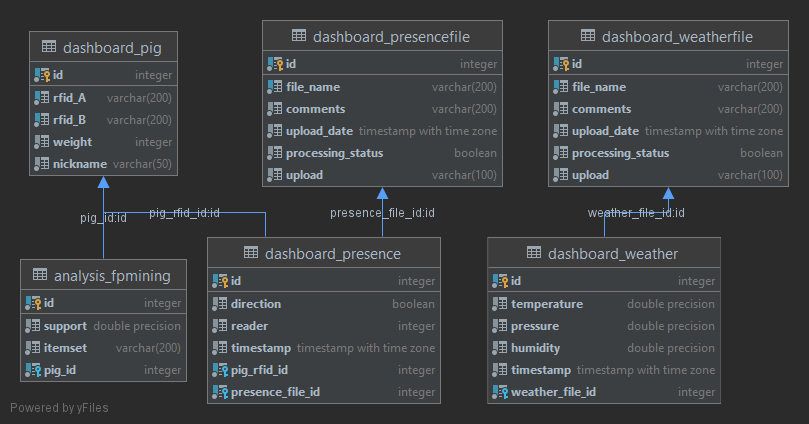
\includegraphics[width=1.0\textwidth]{erd_models}
	\caption{ERD diagram for Django models}
	\label{fig:erd_models}
\end{figure}

\subsection{Migrations}
Migrations are a way to apply incremental changes to the database. After creating or changing an existing model Django
will compare the state of the database schema and the models defined to create a migration file. This migration file
lists the changes needed to be applied to the database schema so that it maps to the models. Migrations can be easily rolled forward
as well as backwards. Furthermore migrations make it easy to have schema changes to be version controlled.

As apps have their own models they also have their own set of migrations. A project can have global migrations as well. Migrations
can populate a database table for example in the case of the Pig table.

After any changes to models, it is necessary to generate migrations by using the command \texttt{python manage.py makemigrations}. Then
the migrations have to be applied by using \texttt{python manage.py migrate}.

\section{Templates}
\label{sec:templates}
Templates are HTML files which can be pre-processed to have dynamic content injected into them. Django ships with it's own
template system called DTL (Django Template Language). It is a very powerful system which allows you to have programmable elements
in the html such as variables and loops. During development if Django is running any changes made to templates are 
automatically shown in the web browser as Django refreshes itself on detecting file changes.

\begin{table}[H]
	\centering
	\begin{tabular}{ | m{0.25\textwidth} | m{0.65\textwidth} | }
		\hline
		\textbf{Template} & \textbf{Description} \\
		\hline \hline
		\emph{index.html} & Landing page of the application. \\
		\hline
		\emph{presence.html} & Data uploading of presence files. \\
		\hline
		\emph{weather.html} & Data uploading of weather files. \\
		\hline
	\end{tabular}
	\caption{Templates in the dashboard app}
	\label{tab:dashboard_templates}
\end{table}

\begin{table}[H]
	\centering
	\begin{tabular}{ | m{0.25\textwidth} | m{0.65\textwidth} | }
		\hline
		\textbf{Template} & \textbf{Description} \\
		\hline \hline
		\emph{dailyanalysis.html} & Scatter plot of Temperature and Humidity \\
		\hline
		\emph{fpmining.html} & FPMining Bar chart for each Pig \\
		\hline
	\end{tabular}
	\caption{Templates in the analysis app}
	\label{tab:analysis_templates}
\end{table}

Template files can be split into multiple files which can then be injected into each other. In the project a global template (main\_template.html)
is defined which contains the navigation, CSS and JavaScript shared by the apps in the project. This template defines the look of the application.
This templates contain the following blocks which can be overridden in the inheriting template files:
\begin{itemize}
	\item Head: Block to include any extra CSS files
	\item Content: Block to include the main output
	\item Scripts: Block to include any extra JS scripts
\end{itemize}

Any inheriting template must have the following basic skeleton. The load static tag is necessary only in the case where 
complete loading of the parent template is necessary for example when using any external JavaScript components such as
Datatables\cite{static_dtl_tag} as in the Upload templates. The scripts and head block is used in Upload template to include JS and CSS for the 
responsive table library Datatables.\cite{datatables} If any block is unused it can be also removed altogether.
\lstset{caption={},label=src:inheriting_skeleton_template}
\begin{lstlisting}[language={HTML}]
	
	

	
	

	
	

	
	
\end{lstlisting}

Incase of a form it is necessary to use the csrf\_token tag for protection
against CSRF and XSS attacks. \cite{django_csrf_protection} If this tag is
omitted then the form will not work at all. The form also has a fallback div
which will be used in case JavaScript is disabled in the browser

\lstset{caption={Upload form in Presence template},label=src:csrf_token}
\begin{lstlisting}[language={HTML}]
	<form action="upload" method="post" class="dropzone" id="textFileDropzone">
		
		<div class="fallback">
			<input name="file" type="file" accept=".txt" multiple/>
		</div>
	</form>
\end{lstlisting}

\subsection{DTL}

DTL allows the use of variables, loops, conditionals and other programmable
logic to be used in a template file. In the content block of
\texttt{presence.html} template the output from the view is a array of Presence
model objects in the variable \texttt{latest\_presence\_files}. Using DTL it is
possible to use a loop to dynamically generate the html required to render all
elements of the array. A conditional is used to set the table column of
Processing status. The url tag takes a name parameter which corresponds to the
name of a defined view. The url tag then generates a link to that particular
view. This way if we have to change URLs then it can be done in the views.py
file and the template will automatically reflect the change. However it is not
possible to define methods or call methods. So all data output should be in its
final form and DTL simply helps to easily manipulate and populate the HTML as
needed.

\lstset{caption={},label=src:presence_upload_template}
\begin{lstlisting}[language={HTML}]

	<tbody>
	
		<tr>
			<td>{{ file.file_name }}</td>
			<td>{{ file.comments }}</td>
			<td>
				
					Processed
				
					In Queue
				
				<a href="" class="icon-block">
					<i style="margin-right: 0.5em;" class="fas fa-redo"></i>
				</a>
			</td>
			<td>{{ file.upload_date }}</td>
		</tr>
	
	</tbody>

\end{lstlisting}

In the content block of \texttt{fpmining.html} template the output from the view is a array of bar graph plots. Using DTL
it is possible to use a loop to dynamically generate the html required to render all elements of the array.

\lstset{caption={},label=src:fpmining_template_loop}
\begin{lstlisting}[language={HTML}]

	
		{{ plot | safe }}
	

\end{lstlisting}

\section{Views}
\label{sec:views}
Views are functions that take a Web request and returns a Web response. The convention is to put views 
in a file called views.py in the application directory. The views themselves may not contain all the logic necessary for processing
and it is preferable to keep large logical code in separate files. Without Views the application would just be a database and template files.
Views are the glue between Models and Templates and make the whole application work seamlessly. Views work by query Models and storing the 
data in a context variable. This is passed to a render function which combines the context with the Template. From there on DTL is used to
generate the required HTML and finally this is passed back to the view which returns the Web response to the URL routing. It is not necessary
to have a template in each view. Some views are trigged by JavaScript elements or form elements and the status is also showing by the triggering
elements so it is enough to return a JSON response which is parsed by the calling element.

\subsection{Dashboard Views}
When the application is opened the user is greeted with 2 cards which show the last time when data files were uploaded.
In index view we query the Presence and Weather model class for the latest row. From the latest rows we extract the timestamp.
This timestamp is subtracted from today's date to get how many days from today the latest data was uploaded. This is combined with
index template in which using DTL we fill the data.

\lstset{caption={Index view for the application dashboard},label=src:index_view}
\begin{lstlisting}[language={Python}]
def index(request):
    max_presence : date = Presence.objects.aggregate(Max('timestamp'))['timestamp__max'].date()
    max_weather : date = Weather.objects.aggregate(Max('timestamp'))['timestamp__max'].date()
    context = {'last_presence_upload': (date.today() - max_presence).days, 'last_weather_upload': (date.today() - max_weather).days}
    return render(request, 'dashboard/index.html', context)
\end{lstlisting}

By browsing to the Upload pages we perform a GET request on the respective URL. The following views are called for a get request.
They query the Model for the latest files and limit the query to 50 results only. In this case in the context we supply the whole
QuerySet returned by the Model query. QuerySet is a array of the respective Model instances. In the template file, these are
looped over and from each instance we can extract all the attribute information as required by the template. Using this approach
our GET views are simplified.

\lstset{caption={GET Uploaded File Views},label=src:get_view}
\begin{lstlisting}[language={Python}]
def presence(request):
    latest_presence_files = PresenceFile.objects.order_by('-upload_date')[:50]
    context = {'latest_presence_files': latest_presence_files}
    return render(request, 'dashboard/presence.html', context)
def weather(request):
    latest_weather_files = WeatherFile.objects.order_by('-upload_date')[:50]
    context = {'latest_weather_files': latest_weather_files}
    return render(request, 'dashboard/weather.html', context)
\end{lstlisting}

When uploading new data files we perform a POST request on the respective URL. We first check if it is indeed a POST request.
Then from the request variable we get the file to be uploaded and store it in a variable. Then we create a new row in the database
for the uploaded file. If this is successful then we call the background task method so that the file is enqueued for processing by
any Celery runner. If all succeeds we return a success JSON response. This response is parsed by the upload form's JavaScript and based
on the response the form shows a tick mark for success or cross in case of failure. For example if the file has been uploaded already
the view will return a error response. This view does not cause a redirect and the user stays on the same page. This view also does not use
a template as it is not required.

\lstset{caption={POST File Upload Views},label=src:post_view}
\begin{lstlisting}[language={Python}]
def presence_upload(request):
    if request.method == 'POST':
        text_file = request.FILES.get('file')
        file = PresenceFile.objects.create(file_name=text_file.name, processing_status=False, upload=text_file)
        processNewPresenceFile.delay(file.id)
        return JsonResponse({'status': 'success'})
    return JsonResponse({'status': 'error'})
def weather_upload(request):
    if request.method == 'POST':
        text_file = request.FILES.get('file')
        file = WeatherFile.objects.create(file_name=text_file.name, processing_status=False, upload=text_file)
        processNewWeatherFile.delay(file.id)
        return JsonResponse({'status': 'success'})
    return JsonResponse({'status': 'error'})

\end{lstlisting}

There may be sometimes a need to process just a single file. The following views are for this purpose. However using these will
return in the webpage being redirected and the user is presented with a JSON response window. This behavior occurs as the view is 
triggered by the user itself and not by any page element.

\lstset{caption={Reprocess File View},label=src:reprocess_view}
\begin{lstlisting}[language={Python}]
def presence_process(request, id):
    return JsonResponse(process_presence_file(id))
def weather_process(request, id):
    return JsonResponse(process_weather_file(id))
\end{lstlisting}

\subsection{Analysis Views}

It can be said that 2 views exist for Analysis app however only one is implemented as a Django view while the other is
implemented as a Dash visualization app. The implemented view is discussed in section \ref{sec:fpmining_example}.

\section{Testing}
\label{sec:testing}

Unit tests have been implemented for processing the uploaded data files. These tests are stored in the tests folder within each app.
The test files are automatically detected and each file name should start with the prefix \texttt{test}.

The set up method is the first method to run before any of the unit tests themselves. In this method we have to setup the database
as per our needs. One should assume that until this point all the migrations of all apps have been applied to the database. Thus keeping 
this in mind we do not need to set up the Pig table as it has already been seeded by \texttt{0002\_seed\_pig\_table.py} migration. However
we do need to supply a text file which will be used by the unit tests. We create a new row in the respective table and fill the data of the
file by using SimpleUploadedFile class which allows us to write the text of the file within the code itself. By using \texttt{b"""} we
have a multiline in which we can simple paste in data from an actual file. This is the recommended and clean way of unit testing a FileField.
\cite{stackoverflow_unittest_filefield}

\lstset{caption={Set Up method for testing},label=src:setup_test}
\begin{lstlisting}[language={Python}]
def setUp(self):
	sample_file = PresenceFile(file_name='20200713_presence.txt')
	sample_file.processing_status = False
	sample_file.upload = SimpleUploadedFile('20200713_presence.txt',b"""+ 1 E2000019991100851580391E 2020-07-13T17:17:35.321 - 4 E20000195206006314302257 2020-07-13T19:39:05.998""")
	sample_file.save()
def setUp(self):
	sample_file = WeatherFile(file_name='20210220_weather.txt')
	sample_file.processing_status = False
	sample_file.upload = SimpleUploadedFile('20210220_weather.txt',	bytes("""temperature: -1.34C, pressure: 1114.18hPa, humidity:  92.09%, time: 2021-02-20T00:00:31.451 temperature: -1.02C, pressure: 1114.19hPa, humidity:  93.36%, time: 2021-02-20T00:20:32.050""" , 'utf-8'))
	sample_file.save()
\end{lstlisting}

The first test cases are for processing valid lines. In testing we found that the data files from the sensors contain
very few errors. The data from the line is extracted and converted into a Presence or Weather model object. Then we check if the values
match. For the presence unit test we also check the foreign key references. In both unit tests the file foreign key is referencing the
file which was inserted into the database by the set up method.

\lstset{caption={Test case for a valid Presence line},label=src:test_process_valid_presence_line}
\begin{lstlisting}[language={Python}]
def test_process_valid_line(self):
	row = process_presence_line('- 4 E20000195206006314302257 2020-07-13T19:39:05.998',	PresenceFile.objects.first())
	self.assertEqual(False, row.direction)
	self.assertEqual(4, row.reader)
	self.assertEqual(Pig.objects.get(pk=3), row.pig_rfid)
	self.assertEqual(datetime.fromisoformat('2020-07-13T19:39:05.998'), row.timestamp)
\end{lstlisting}

\lstset{caption={Test case for a valid Weather line},label=src:test_process_valid_weather_line}
\begin{lstlisting}[language={Python}]
def test_process_valid_line(self):
	row = process_weather_line('temperature: -1.34C, pressure: 1114.18hPa, humidity:  92.09%, time: 2021-02-20T00:00:31.451',WeatherFile.objects.first())
	self.assertEqual(-1.34, row.temperature)
	self.assertEqual(1114.18, row.pressure)
	self.assertEqual(92.09, row.humidity)
	self.assertEqual(datetime.fromisoformat('2021-02-20T00:00:31.451'), row.timestamp)
\end{lstlisting}

In the unit tests for incorrect data lines the tested method should throw an exception and the exception should have in it's 
message the detail about why and where the line is incorrect. This is very important as it will help us to identify the error
in the text file itself. 

The method \texttt{assertRaisesRegex} is used as it is the only method which also test the returned 
exception message and not only the exception. ValueError exception is used because it is the primary exception raised when faulty
data input is detected. Each assertion contains a single different error for each attribute of the input line. The format of each attribute is also tested 
for example the RFID can only contain alphanumeric characters. The assertion messages have to be in the regex format otherwise the 
\texttt{assertRaisesRegex} method will not correctly compared the returned exception message and the comparison message.

\lstset{caption={Test case for an invalid Presence line},label=src:test_process_invalid_presence_line}
\begin{lstlisting}[language={Python}]
def test_process_invalid_line(self):
	self.assertRaisesRegex(ValueError, 'Empty Input', validate_presence_line, '')
	self.assertRaisesRegex(ValueError, r'^Expected \+ or - for direction$', validate_presence_line, '# 4 E20000195206006314302257 2020-07-13T19:39:05.998')
	self.assertRaisesRegex(ValueError, r'^Incorrect reader number format$', validate_presence_line, '+ 99 E20000195206006314302257 2020-07-13T19:39:05.998')
	self.assertRaisesRegex(ValueError, r'^Incorrect RFID format$', validate_presence_line, '+ 4 E2!@#$%^&*()7 2020-07-13T19:39:05.998')
	self.assertRaisesRegex(ValueError, r'^Invalid DateTime$', validate_presence_line, '+ 4 E20000195206006314302257 ABCD-07-13W19:39T:05.998')
	self.assertRaisesRegex(ValueError, r'^RFID does not exist$', validate_presence_line, '+ 4 E99999999999999999999999 2020-07-13T19:39:05.998')
\end{lstlisting}

Empty input and out of 
bound input is also tested for example the value of Humidity should be between 0\% and 100\%.

\lstset{caption={Test case for a invalid Weather line},label=src:test_process_invalid_weather_line}
\begin{lstlisting}[language={Python}]
def test_process_invalid_line(self):
	self.assertRaisesRegex(ValueError, 'Empty Input', validate_weather_line, '')
	self.assertRaisesRegex(ValueError, r'^Out of Range Temperature. Limit is 50.00C to -50.00C$',validate_weather_line, 'temperature: -1000.34C, pressure: 1114.18hPa, humidity:  92.09%, time: 2021-02-20T00:00:31.451')
	self.assertRaisesRegex(ValueError, r'^Out of Range Pressure. Limit is 1000.00hPa to 1500.00hPa$', validate_weather_line, 'temperature: -1.34C, pressure: 5000.18hPa, humidity:  92.09%, time: 2021-02-20T00:00:31.451')
	self.assertRaisesRegex(ValueError, r'^Out of Range Humidity. Limit is 0.00% to 100.00%$', validate_weather_line, 'temperature: -1.34C, pressure: 1114.18hPa, humidity:  101.00%, time: 2021-02-20T00:00:31.451')
\end{lstlisting}

\section{GitHub Continuous Integration}
CI is the practice of merging work into a main branch regularly. To obtain this
goal GitHub actions have been set up for this repository which build the project
and run the unit tests on a fresh docker container. In this method multiple branches
can exist which contain work for different features and it assures that any breaking changes
can be quickly detected and fixed.

The docker container runs the latest ubuntu OS on which python 3.8 is installed.
Afterwards PostgreSQL is set up with the provided credentials. These credentials are
also present in the settings.py file. Next all required python packages are installed and then
for the purposes of logging the migrations are logged to the console for inspection. Afterwards
the unit tests are run and if everything is successful then the whole action passes for the commit.
These action occur on every push for the latest commit. The upload directory's permissions need to be
set as the unit tests cause some file operations to take place which would fail without the proper
permissions.

\lstset{caption={GitHub actions for the
project},label=src:github_actions}
\begin{lstlisting}[language={Python}]
runs-on: ubuntu-latest
services:
	postgres:
		POSTGRES_USER: postgres
		POSTGRES_PASSWORD: postgres
		POSTGRES_DB: github_actions
	- name: Run migrations
	run: |
		python manage.py makemigrations
		python manage.py showmigrations
		python manage.py migrate
	- name: Run Tests
	run: |
		sudo mkdir /media/uploads
		sudo chown -R $USER:$USER /media/uploads
		python manage.py test -v 2
\end{lstlisting}

The logs can be found under actions tab on GitHub. If there are any artifacts
they are also available for download. In case some action fails the logs can be
used to diagnose the issue. In large projects the build takes some amount of
time and the developer's system might not be clean so it is preferred to always
use the CI to build and run the tests.

\begin{figure}[H]
	\centering
	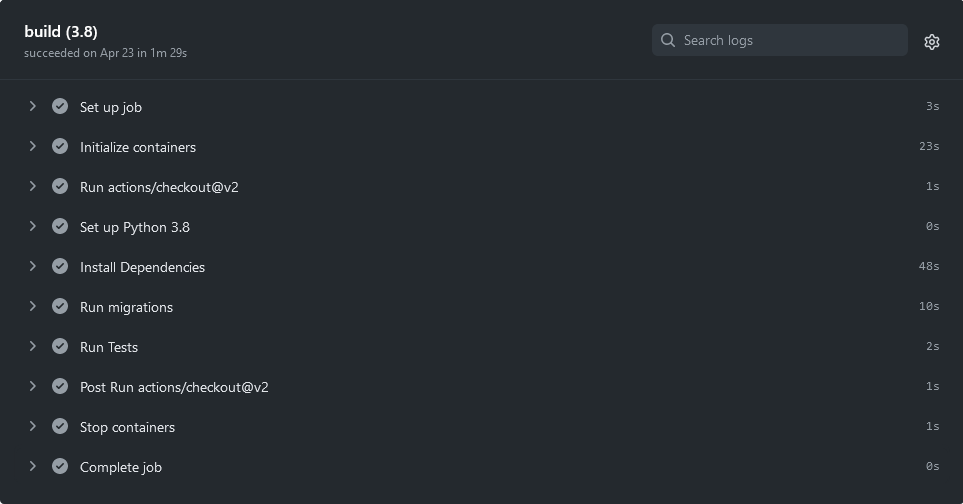
\includegraphics[width=1.0\textwidth]{github_action_log}
	\caption{GitHub CI action log}
	\label{fig:github_action_log}
\end{figure}

\section{FPMining Example}
\label{sec:fpmining_example}
A data analysis solution was developed by Rohit \cite{rohit_github} and it is included in the project as an example of extending the application.
In summary it tells us when the pig likes to visit a certain area and in what weather conditions.

The first step is to analyze the solution and identify the critical inputs/outputs and processing methods. It is necessary to 
isolate the processing so that it can be directly moved into the project. Next the most difficult part of the process is tackled which
is to provide the processing methods with the same input from our Django models. Afterwards it is necessary to develop a Dash or plotly app
to visualize the output.

\subsection{Isolating the logic}
The logical part of the solution is easily identified in the original solution by looking at the flow
of the program while debugging. The \texttt{FPGrowth} method is the core logic and it was moved into the project
after including the python packages required (Numpy, Pandas, mlxtend) in the project. The main data input is the dataset parameter and
the other parameters are of Double type. Now it is necessary to generate the dataset in the correct format from our Django models for this
method.

\lstset{caption={Core logic method of the solution},label=src:FPGrowth}
\begin{lstlisting}[language={Python}]
def FPGrowth(dataset, min_support, min_length, min_support_of_custom_itemsets):
    frequent_itemsets = fpgrowth(df=dataset, min_support=min_support, use_colnames=True, max_len=None)
    frequent_itemsets['length'] = frequent_itemsets['itemsets'].apply(lambda x: len(x))
    freq_items = frequent_itemsets[(frequent_itemsets['length'] >= min_length) & (frequent_itemsets['support'] >= min_support_of_custom_itemsets)]
    return freq_items
\end{lstlisting}

\subsection{Generating Input data using Django Models}
In the original script Rohit processed raw text files and saved the intermediate output in text files as well.
The disadvantage of this approach is that it takes a long processing time if the data is of large size. Furthermore
using text files he had to write a lot of helper code to perform comparisons and sorting of data. This is not required in Django
as we already leverage the power of SQL but also on top of it the Django ORM.

Given a Pig model ID we find every entry (+) Presence row associated with that pig ID. Next we try to find within 30 minutes the last
exit(-) Presence row for the selected pig. By doing this we decrease the size of the dataset considerable and smooth out the data.
This give us a time framed dataset which we combine with the first Weather row whose timestamp is in the 30 minutes timeframe.
In the end we have a list of entry and exit of a pig with the appended weather conditions.

\lstset{caption={Combine Presence with Weather according to closest time},label=src:generate_dataframe_for_FPGrowth}
\begin{lstlisting}[language={Python}]
def summarizedEntryExit(primary_key) -> list:
    dataset = []
    processed_until_timestamp: datetime = datetime.datetime(2000, 1, 1)
    for _presence in Presence.objects.filter(direction=True, pig_rfid=primary_key):
        if processed_until_timestamp > _presence.timestamp:
            continue
        start_of_30_minutes = _presence.timestamp
        end_of_30_minutes = start_of_30_minutes + datetime.timedelta(minutes=30)
        processed_until_timestamp = end_of_30_minutes
        exit_of_pig = Presence.objects.filter(timestamp__range=(start_of_30_minutes, end_of_30_minutes), direction=False, pig_rfid=_presence.pig_rfid).order_by('timestamp')
        furthest_exit_of_pig = exit_of_pig.last()
        closest_weather = Weather.objects.filter(timestamp__range=(start_of_30_minutes, end_of_30_minutes)).first()
        if not closest_weather:
            continue
        dataset.append([_presence, furthest_exit_of_pig, closest_weather])
    return dataset
\end{lstlisting}

\subsection{Creating Celery Task and Model for output}
The next step is to have the processing automated as soon as new data is input into the system. To achieve this we need to
declare a Celery \@shared\_task set up. Furthermore as the task will run it's output needs to be stored as well so that 
it can be directly visualized by the front-end.

Remember that the FPGrowth method needs to run for each pig so in the task we loop over all distinct Pig model rows,
generate the dataset for each Pig and then apply the FPGrowth method. After discussion with the author the key output columns
were identified and then they are saved to the database. At this point the parameters of the method are set. If necessary they can
be generated dynamically but for the purpose of the current application they were set to fixed values by the author. If needed the
Celery task method can be provided with a JSON array with the required parameters.

The model is very simple consisting of a Pig foreign key, float attribute for support and char field for storing the itemsets array.

\lstset{caption={\makeatletter shared\_task method for background processing},label=src:processFPGrowthForWholeDataset}
\begin{lstlisting}[language={Python}]
for pig in pigs_in_data:
	df = generate_dataframe_for_FPGrowth(pig.pig_rfid)
	processed_data_df = FPGrowth(dataset=df, min_support=0.1, min_length=3, min_support_of_custom_itemsets=0.1)
	for index, row in processed_data_df.iterrows():
		db_row = FPMining()
		db_row.pig_id = pig.pig_rfid_id
		db_row.support = round(row["support"] * 100, 2)
		db_row.itemset = ', '.join(row["itemsets"])
		db_row.save()
\end{lstlisting}

\subsection{Visualizing the Output}
Since now we know the database model of the output we can decide how to visualize the data. In this example
the author already decided that bar charts should be used. Now since due to the large number of bar charts it would not be feasible
to create a Dash app since it would be instantiated on the launch of the application and consume many resources. Also the bar
charts need not to be updated and so we further do not need to leverage Dash.

It is better to use a Django view to create Plotly apps on the fly as the user requests and stich all the apps in a single
template. For each pig we generate a figure to which a Bar trace is added containing the data. This figure is used by the method
plot to generate HTML code required to render the graphics. By setting output type to div, \texttt{plot} method returns HTML
code. We disable inclusion of plotly\.js JavaScript library since it is included
once in the template itself. Including the library again and again will slow down the loading of the page. 

The go.Bar method requires the data for the x and y axis. We query the FPMining model and get the results in a QuerySet by using \texttt{values\_list}
method. The go.Bar method only accepts input of type List so we need to convert the QuerySet to a list.
The layout variable is give a dictionary with the key-value pair of the title of the graph so that each graph can be identified by the Pig nickname.
The render method is passed the template as well as the array of plots in context variable to generate the Web response for the view.

\lstset{caption={\makeatletter shared\_task method for background processing},label=src:simpleFPmining_view}
\begin{lstlisting}[language={Python}]
for pig in pigs_in_data:
	trace = go.Bar(x=list(all_rows.filter(pig_id=pig.pig_id).values_list('itemset', flat=True)), y=list(all_rows.filter(pig_id=pig.pig_id).values_list('support', flat=True)))
	layout = dict(title=pig.pig.nickname,)
	fig = go.Figure(data=[trace], layout=layout)
	plot_div = plot(fig, output_type='div', include_plotlyjs=False)
	plots.append(plot_div)
return render(request, "analysis/fpmining.html", context={'plots': plots})
\end{lstlisting}